%%%%%%%%%%%%%%%%%%%%%%%%%%%%%%%%%%%%%%%%%%%%%%%%%%%%%%%%%%%%%%%%%%%%%%%%%%%%%%%
% Derivation Attempt v3: Can κ₅² be fixed by σ?
% Dimensional analysis + junction condition consistency
%
% Status: WORKING / OPEN
%%%%%%%%%%%%%%%%%%%%%%%%%%%%%%%%%%%%%%%%%%%%%%%%%%%%%%%%%%%%%%%%%%%%%%%%%%%%%%%
\documentclass[11pt,a4paper]{article}

\usepackage[utf8]{inputenc}
\usepackage[T1]{fontenc}
\usepackage{amsmath,amssymb,amsthm}
\usepackage{geometry}
\geometry{margin=2.5cm}
\usepackage{hyperref}
\hypersetup{colorlinks=true, linkcolor=blue!60!black, citecolor=blue!60!black}
\usepackage{booktabs}
\usepackage{enumitem}
\usepackage{tikz}
\usetikzlibrary{arrows.meta, positioning}
\usepackage{tcolorbox}
\tcbuselibrary{skins,breakable}

% Epistemic tags
\newcommand{\tagBL}{\textcolor{blue!70!black}{[BL]}}
\newcommand{\tagI}{\textcolor{green!50!black}{[I]}}
\newcommand{\tagP}{\textcolor{orange!80!black}{[P]}}
\newcommand{\tagOPEN}{\textcolor{red!70!black}{[OPEN]}}
\newcommand{\tagDc}{\textcolor{purple!70!black}{[Dc]}}

% Box environments
\newtcolorbox{statusbox}{
  colback=yellow!5!white,
  colframe=yellow!50!black,
  breakable
}

\newtcolorbox{dimbox}{
  colback=blue!5!white,
  colframe=blue!50!black,
  title=Dimensional Ledger,
  breakable
}

\newtcolorbox{resultbox}{
  colback=green!5!white,
  colframe=green!50!black,
  breakable
}

\newtcolorbox{nogobox}{
  colback=red!5!white,
  colframe=red!50!black,
  title=Underdetermination Statement,
  breakable
}

\newtheorem{proposition}{Proposition}

\title{\textbf{EDC BLOCK-003 (Derivation Attempt v3):}\\[0.3em]
Can $\kappa_5^2$ Be Fixed by $\sigma$?\\[0.5em]
\large Derivation attempt / program note; not a results paper}
\author{EDC Research Program}
\date{2026-02-02\\[0.3em]\small\textit{Status: WORKING / OPEN}}

\begin{document}

\maketitle

%===============================================================================
\section{Executive Summary}
\label{sec:summary}
%===============================================================================

\begin{statusbox}
\textbf{Question:} Can the 5D gravitational coupling $\kappa_5^2$ be determined by the brane tension $\sigma$ alone, without importing additional scales?

\textbf{Outcome: INCONCLUSIVE.}

Dimensional analysis permits $\kappa_5^2 = C \cdot \sigma^{-3/4}$ (in natural units), where $C$ is an undetermined dimensionless constant.
This relation is consistent with Israel junction conditions.
However, $\sigma$ alone cannot fix $C$; there exists a residual normalization freedom.

\textbf{Conclusion:} $\sigma$ determines a natural length scale $\ell_\sigma \sim \sigma^{-1/4}$, but $\kappa_5^2$ requires an additional input to be fully specified.
BLOCK-003 remains OPEN.
\end{statusbox}

%===============================================================================
\section{Setup: The 5D Action}
\label{sec:setup}
%===============================================================================

\paragraph{Action \tagBL{}.}
The total gravitational action is:
\begin{equation}
    S = \underbrace{\frac{1}{2\kappa_5^2} \int_{\mathcal{M}^5} d^5X \sqrt{-g} \left( R^{(5)} - 2\Lambda_5 \right)}_{S_{\text{bulk}}}
    + \underbrace{\frac{1}{\kappa_5^2} \int_{\partial\mathcal{M}} d^4x \sqrt{-h} \, K}_{S_{\text{GHY}}}
    - \underbrace{\sigma \int_\Sigma d^4x \sqrt{-\gamma}}_{S_{\text{brane}}}.
    \label{eq:action}
\end{equation}

\paragraph{Parameters \tagBL{}/\tagP{}.}
\begin{itemize}[nosep]
    \item $\kappa_5^2 = 8\pi G_5$: 5D gravitational coupling (to be determined).
    \item $\Lambda_5$: bulk cosmological constant (set to zero for simplicity in this analysis).
    \item $\sigma$: brane tension (energy per unit 4-volume, i.e., energy/area in static slicing).
\end{itemize}

\paragraph{Goal.}
Determine whether $\kappa_5^2$ can be expressed as a function of $\sigma$ alone:
\begin{equation}
    \kappa_5^2 \stackrel{?}{=} f(\sigma).
    \label{eq:goal}
\end{equation}

%===============================================================================
\section{Dimensional Analysis}
\label{sec:dimensions}
%===============================================================================

\begin{dimbox}
\textbf{Natural units} ($c = \hbar = 1$):

All quantities expressed in powers of length $L$.
\begin{center}
\renewcommand{\arraystretch}{1.2}
\begin{tabular}{lll}
\toprule
\textbf{Quantity} & \textbf{Dimension} & \textbf{Notes} \\
\midrule
$[\sigma]$ & $L^{-4}$ & Energy/area = $M \cdot L^{-2}$ = $L^{-1} \cdot L^{-2}$ = $L^{-4}$ \\
$[G_5]$ & $L^{3}$ & 5D Newton constant \\
$[\kappa_5^2]$ & $L^{3}$ & Since $\kappa_5^2 = 8\pi G_5$ \\
$[\Lambda_5]$ & $L^{-2}$ & Cosmological constant \\
$[K_{\mu\nu}]$ & $L^{-1}$ & Extrinsic curvature \\
\bottomrule
\end{tabular}
\end{center}
\end{dimbox}

\paragraph{Key observation \tagDc{}.}
From $\sigma$ alone, we can construct a characteristic length:
\begin{equation}
    \ell_\sigma \equiv \sigma^{-1/4}, \qquad [\ell_\sigma] = L.
    \label{eq:ell_sigma}
\end{equation}
This is the \emph{only} length scale derivable from $\sigma$.

\paragraph{Dimensional possibility for $\kappa_5^2$ \tagDc{}.}
Since $[\kappa_5^2] = L^3$, we need three powers of length.
Using $\ell_\sigma$:
\begin{equation}
    \boxed{\kappa_5^2 = C \cdot \ell_\sigma^3 = C \cdot \sigma^{-3/4},}
    \label{eq:kappa5_dimensional}
\end{equation}
where $C$ is a \emph{dimensionless constant} not determined by dimensional analysis.

\begin{resultbox}
\textbf{Dimensional result:}
The relation $\kappa_5^2 \propto \sigma^{-3/4}$ is the unique dimensionally consistent possibility if $\sigma$ is the only input.
However, the proportionality constant $C$ is not fixed.
\end{resultbox}

%===============================================================================
\section{Attempt A: Test Consistency with Junction Conditions}
\label{sec:attempt_A}
%===============================================================================

\paragraph{Israel junction conditions \tagBL{}.}
At the brane $\Sigma$, the jump in extrinsic curvature satisfies:
\begin{equation}
    [K_{\mu\nu}] - [K] \gamma_{\mu\nu} = -\kappa_5^2 \left( S_{\mu\nu} - \frac{1}{3} S \gamma_{\mu\nu} \right).
    \label{eq:israel}
\end{equation}

\paragraph{Pure tension brane \tagBL{}.}
For $S_{\mu\nu} = -\sigma \gamma_{\mu\nu}$ (tension only), with $S = -4\sigma$:
\begin{equation}
    [K_{\mu\nu}] - [K] \gamma_{\mu\nu} = -\kappa_5^2 \left( -\sigma + \frac{4\sigma}{3} \right) \gamma_{\mu\nu} = -\frac{\kappa_5^2 \sigma}{3} \gamma_{\mu\nu}.
    \label{eq:israel_tension}
\end{equation}
Taking the trace ($\gamma^{\mu\nu} \gamma_{\mu\nu} = 4$):
\begin{equation}
    -3[K] = -\frac{4\kappa_5^2 \sigma}{3} \quad \Rightarrow \quad [K] = \frac{4\kappa_5^2 \sigma}{9}.
\end{equation}
Thus the curvature scale is:
\begin{equation}
    k \equiv [K] \sim \kappa_5^2 \sigma.
    \label{eq:k_scale}
\end{equation}

\paragraph{Substitute the dimensional ansatz \tagDc{}.}
Using $\kappa_5^2 = C \sigma^{-3/4}$:
\begin{equation}
    k \sim C \sigma^{-3/4} \cdot \sigma = C \sigma^{1/4}.
    \label{eq:k_substituted}
\end{equation}
The corresponding curvature length is:
\begin{equation}
    \ell_k \equiv k^{-1} \sim C^{-1} \sigma^{-1/4} = C^{-1} \ell_\sigma.
    \label{eq:ell_k}
\end{equation}

\begin{resultbox}
\textbf{Consistency check: PASS.}

The ansatz $\kappa_5^2 = C \sigma^{-3/4}$ is dimensionally consistent with the Israel junction conditions.
The curvature scale $k \sim \sigma^{1/4}$ and length $\ell_k \sim \ell_\sigma$ are well-defined for any $C > 0$.

\textbf{But:} The constant $C$ remains undetermined.
\end{resultbox}

%===============================================================================
\section{Attempt B: Can $C$ Be Fixed by Normalization?}
\label{sec:attempt_B}
%===============================================================================

\paragraph{The residual freedom \tagI{}.}
The action \eqref{eq:action} has a normalization freedom:
\begin{itemize}[nosep]
    \item Rescaling $g_{AB} \to \lambda^2 g_{AB}$ changes $\sqrt{-g}$, $R$, and $K$.
    \item Correspondingly, $\kappa_5^2$ and $\sigma$ can be redefined to keep the action invariant.
\end{itemize}
This is a \emph{coordinate/unit choice}, not physics.

\paragraph{Can EDC fix $C$? \tagOPEN{}.}
For $C$ to be determined, EDC would need to provide one of:
\begin{enumerate}[nosep]
    \item A canonical definition of $\sigma$ in terms of a fundamental action density (with fixed normalization).
    \item An independent equation relating $\kappa_5^2$ to $\sigma$ (beyond dimensional consistency).
    \item A matching condition to another sector (e.g., EM) that breaks the freedom.
\end{enumerate}
\textbf{None of these is currently available in EDC.}

\begin{nogobox}
\begin{proposition}[Underdetermination]
\label{prop:underdetermination}
Let $\sigma$ be the only input parameter with $[\sigma] = L^{-4}$.
Then:
\begin{enumerate}
    \item The unique dimensionally consistent relation is $\kappa_5^2 = C \cdot \sigma^{-3/4}$.
    \item The constant $C$ cannot be fixed by $\sigma$ alone.
    \item The junction conditions are satisfied for any $C > 0$, with curvature scale $k = C \sigma^{1/4}$.
\end{enumerate}
Therefore, $\sigma$ alone does not determine $\kappa_5^2$ uniquely.
\end{proposition}
\end{nogobox}

%===============================================================================
\section{What Would Fix $C$?}
\label{sec:fix_C}
%===============================================================================

\paragraph{Possible additional inputs \tagOPEN{}.}
\begin{center}
\renewcommand{\arraystretch}{1.2}
\begin{tabular}{p{3.5cm}p{2cm}p{6cm}}
\toprule
\textbf{Input} & \textbf{Dimension} & \textbf{How it could fix $C$} \\
\midrule
$\Lambda_5$ (bulk cosm.\ const.) & $L^{-2}$ & Provides second scale; $C$ from $\sigma / \Lambda_5^2$ \\
$\ell_5$ (fundamental 5D length) & $L$ & Direct: $\kappa_5^2 \sim \ell_5^3$; then $C = (\ell_5 / \ell_\sigma)^3$ \\
$M_5$ (5D Planck mass) & $L^{-1}$ & $\kappa_5^2 = M_5^{-3}$; relates to $\sigma$ via dynamics \\
Matching to $G_N$ & --- & Circular (prohibited) \\
\bottomrule
\end{tabular}
\end{center}

\paragraph{EDC-internal candidates \tagI{}.}
If EDC defines $\sigma$ via a specific microscopic mechanism (e.g., $\sigma = 2\pi R_\xi^2 \rho_P$ for some pressure $\rho_P$), then additional structure enters.
But this is not a $\sigma$-only derivation; it imports the scale $R_\xi$.

%===============================================================================
\section{Dependency Schematic}
\label{sec:schematic}
%===============================================================================

\begin{figure}[ht]
\centering
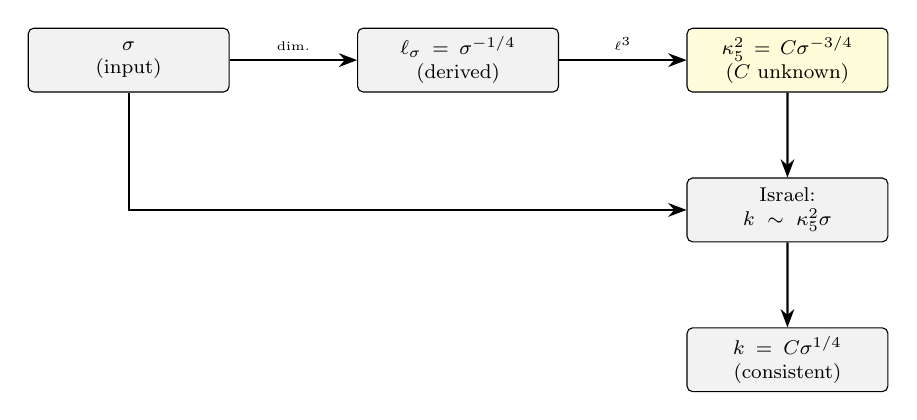
\begin{tikzpicture}[>=Stealth, node distance=1.8cm, scale=0.9, transform shape,
    box/.style={rectangle, draw, fill=gray!10, text width=2.6cm, text centered,
                minimum height=0.9cm, font=\footnotesize, rounded corners=2pt},
    openbox/.style={rectangle, draw, fill=yellow!15, text width=2.6cm, text centered,
                minimum height=0.9cm, font=\footnotesize, rounded corners=2pt},
    arrow/.style={->, thick}]

    \node[box] (sigma) {$\sigma$\\(input)};
    \node[box, right=of sigma] (ell) {$\ell_\sigma = \sigma^{-1/4}$\\(derived)};
    \node[openbox, right=of ell] (kappa) {$\kappa_5^2 = C \sigma^{-3/4}$\\($C$ unknown)};
    \node[box, below=1.2cm of kappa] (israel) {Israel:\\$k \sim \kappa_5^2 \sigma$};
    \node[box, below=1.2cm of israel] (k) {$k = C \sigma^{1/4}$\\(consistent)};

    \draw[arrow] (sigma) -- (ell) node[midway, above, font=\tiny] {dim.};
    \draw[arrow] (ell) -- (kappa) node[midway, above, font=\tiny] {$\ell^3$};
    \draw[arrow] (kappa) -- (israel);
    \draw[arrow] (sigma) |- (israel);
    \draw[arrow] (israel) -- (k);
\end{tikzpicture}
\caption{Derivation schematic (program overview; not a result). The constant $C$ remains undetermined by $\sigma$ alone.}
\label{fig:schematic}
\end{figure}

%===============================================================================
\section{Outcome}
\label{sec:outcome}
%===============================================================================

\begin{nogobox}
\textbf{Outcome: INCONCLUSIVE.}

\begin{itemize}[nosep]
    \item \textbf{Dimensional analysis:} $\kappa_5^2 = C \sigma^{-3/4}$ is the unique consistent form.
    \item \textbf{Junction conditions:} Satisfied for any $C > 0$.
    \item \textbf{Constant $C$:} Not fixed by $\sigma$ alone; requires additional input.
    \item \textbf{No-go:} $\sigma$ determines $\ell_\sigma$ but not $\kappa_5^2$ uniquely.
\end{itemize}

\textbf{Missing element:} An independent scale or normalization condition to fix $C$.
\end{nogobox}

%===============================================================================
\section{Bridge to BLOCK-003}
\label{sec:bridge}
%===============================================================================

From derivation\_v2, setting $L = R_\xi$ gives:
\begin{equation}
    G_N = \frac{\kappa_5^2}{6\pi R_\xi}.
\end{equation}
Substituting $\kappa_5^2 = C \sigma^{-3/4}$:
\begin{equation}
    G_N = \frac{C \sigma^{-3/4}}{6\pi R_\xi}.
    \label{eq:GN_with_C}
\end{equation}
This still contains the undetermined constant $C$.

\textbf{Conclusion:} Even combining derivation\_v2 ($L = R_\xi$) with derivation\_v3 ($\kappa_5^2 \propto \sigma^{-3/4}$), BLOCK-003 remains OPEN because $C$ is not fixed.

The missing link is now narrowed to: \textbf{fix $C$} (or equivalently, provide an independent length scale that sets $\kappa_5^2$ absolutely).

%===============================================================================
\section{Conclusion}
\label{sec:conclusion}
%===============================================================================

\begin{enumerate}[nosep]
    \item $\sigma$ provides a natural length scale $\ell_\sigma = \sigma^{-1/4}$.
    \item Dimensional analysis gives $\kappa_5^2 = C \sigma^{-3/4}$ as the unique consistent form.
    \item The Israel junction conditions are satisfied for any $C > 0$.
    \item The constant $C$ cannot be fixed by $\sigma$ alone.
    \item \textbf{BLOCK-003 remains OPEN}; the missing element is narrowed to fixing $C$.
\end{enumerate}

\paragraph{Next step (out of scope).}
Investigate whether EDC's definition of $\sigma$ (via membrane geometry or pressure integration) provides the normalization needed to fix $C$.

\end{document}
